% =====================================================================
%  Chapitre 3 -- Architecture d'un réseau convolutif
%  Partie b : pooling, flatten, couches denses, softmax, entropie croisée
%             et pipeline complet d'un CNN
% =====================================================================

\begin{frame}{Plan de cette partie}
\begin{columns}[t]
\begin{column}{0.48\textwidth}
\begin{kbox}[Les cinq étapes de l'assemblage]
\begin{enumerate}
  \item Le \textbf{pooling} : réduire et rendre robuste.
  \item Le \textbf{global average pooling}.
  \item Le \textbf{flatten} : du tenseur au vecteur.
  \item Les \textbf{couches denses} et la \textbf{softmax}.
  \item Le \textbf{pipeline complet} : conv $\to$ ReLU $\to$ pool $\to \cdots$.
\end{enumerate}
\end{kbox}
\end{column}
\begin{column}{0.48\textwidth}
\begin{ebox}[Ce que vous saurez faire]
\begin{itemize}
  \item Calculer une opération de max pooling et de moyenne pooling à la main.
  \item Expliquer pourquoi le pooling n'a aucun paramètre.
  \item Passer d'un tenseur $H\times W\times C$ à un vecteur.
  \item Transformer des scores en probabilités avec la softmax.
  \item Dérouler le chemin d'une image jusqu'à la classe prédite.
\end{itemize}
\end{ebox}
\end{column}
\end{columns}
\vspace{1mm}

% [fix] bloc deplace
\end{frame}
\begin{frame}{Plan de cette partie (suite)}
\begin{wbox}[La ligne d'assemblage]
Extraction de motifs par la convolution, non-linéarité par ReLU, résumé spatial
par le pooling, décision par les couches denses. Ce chapitre met ces briques bout à bout.
\end{wbox}
\end{frame}

\begin{frame}{Le pooling : pourquoi réduire la taille ?}
\begin{columns}[t]
\begin{column}{0.52\textwidth}
\begin{itemize}
  \item Après les convolutions, les cartes restent \textbf{grandes} :
  beaucoup de valeurs pour peu d'information utile.
  \item Le pooling \textbf{résume} chaque petit voisinage par une seule valeur.
  \item Effet : la carte spatiale rétrécit, le nombre de canaux \textbf{ne change pas}.
  \item Deux bénéfices : moins de calcul pour les couches suivantes, et une
  \textbf{robustesse} aux petits décalages du motif.
\end{itemize}
\begin{kbox}[Aucun paramètre]
Le pooling n'apprend \textbf{rien} : c'est une règle fixe (un maximum, une
moyenne). Le nombre de paramètres d'un réseau vient uniquement des convolutions
et des couches denses.
\end{kbox}
\end{column}
\begin{column}{0.44\textwidth}
\begin{ebox}[Dimensionnement]
Avec une fenêtre $2 \times 2$ et un pas de $2$, une carte
$H \times W$ devient $\tfrac{H}{2} \times \tfrac{W}{2}$ : la surface est
divisée par $4$.
\end{ebox}
\begin{wbox}[Ne pas confondre]
Le pooling \textbf{réduit} la résolution. Il ne remplace pas la convolution :
il ne détecte aucun motif, il agrège ceux déjà détectés.
\end{wbox}
\end{column}
\end{columns}
\end{frame}

\begin{frame}{Max pooling $2\times 2$ : le calcul à la main}
\begin{columns}[t]
\begin{column}{0.44\textwidth}
\[
M=\begin{bmatrix}
1 & 2 & 5 & 3\\
4 & 9 & 2 & 1\\
7 & 3 & 8 & 6\\
2 & 1 & 4 & 5
\end{bmatrix}
\]
\begin{itemize}
  \item Fenêtre $2 \times 2$, pas de $2$ : quatre blocs disjoints.
  \item On garde le \textbf{maximum} de chaque bloc.
\end{itemize}
\end{column}
\begin{column}{0.52\textwidth}
\begin{ebox}[Les quatre blocs]
Bloc haut-gauche $\begin{smallmatrix}1&2\\4&9\end{smallmatrix}$
$\to \max = 9$ ;
bloc haut-droit $\begin{smallmatrix}5&3\\2&1\end{smallmatrix}$
$\to \max = 5$ ;
bloc bas-gauche $\begin{smallmatrix}7&3\\2&1\end{smallmatrix}$
$\to \max = 7$ ;
bloc bas-droit $\begin{smallmatrix}8&6\\4&5\end{smallmatrix}$
$\to \max = 8$.
\end{ebox}
\[
\mathrm{MaxPool}_{2\times2}(M)=
\begin{bmatrix}
9 & 5\\
7 & 8
\end{bmatrix}
\]
\end{column}
\end{columns}
\vspace{1mm}
\begin{kbox}[Lecture]
$4 \times 4 = 16$ valeurs deviennent $2 \times 2 = 4$. La plus forte réponse
de chaque région est conservée : c'est elle qui traduit la présence du motif.
\end{kbox}
\end{frame}

\begin{frame}{Average pooling $2\times 2$ : le calcul à la main}
\begin{columns}[t]
\begin{column}{0.52\textwidth}
\begin{ebox}[Les quatre moyennes]
Bloc haut-gauche : $(1+2+4+9)/4 = 16/4 = 4$.

Bloc haut-droit : $(5+3+2+1)/4 = 11/4 = 2{,}75$.

Bloc bas-gauche : $(7+3+2+1)/4 = 13/4 = 3{,}25$.

Bloc bas-droit : $(8+6+4+5)/4 = 23/4 = 5{,}75$.
\end{ebox}
\end{column}
\begin{column}{0.44\textwidth}
\[
\mathrm{AvgPool}_{2\times2}(M)=
\begin{bmatrix}
4 & 2{,}75\\
3{,}25 & 5{,}75
\end{bmatrix}
\]
\begin{itemize}
  \item Mêmes dimensions que le max pooling, mais une valeur \textbf{lissée}.
  \item Le max isole le pic ; la moyenne tient compte de tout le bloc.
\end{itemize}
\end{column}
\end{columns}
\vspace{1mm}
\begin{kbox}[Comparaison directe]
Sur la même matrice : max pooling
$\begin{psmallmatrix}9&5\\7&8\end{psmallmatrix}$, moyenne pooling
$\begin{psmallmatrix}4&2{,}75\\3{,}25&5{,}75\end{psmallmatrix}$.
En pratique, le \textbf{max} domine dans les CNN de classification.
\end{kbox}
\end{frame}

\begin{frame}{Le pooling en images}
\begin{center}
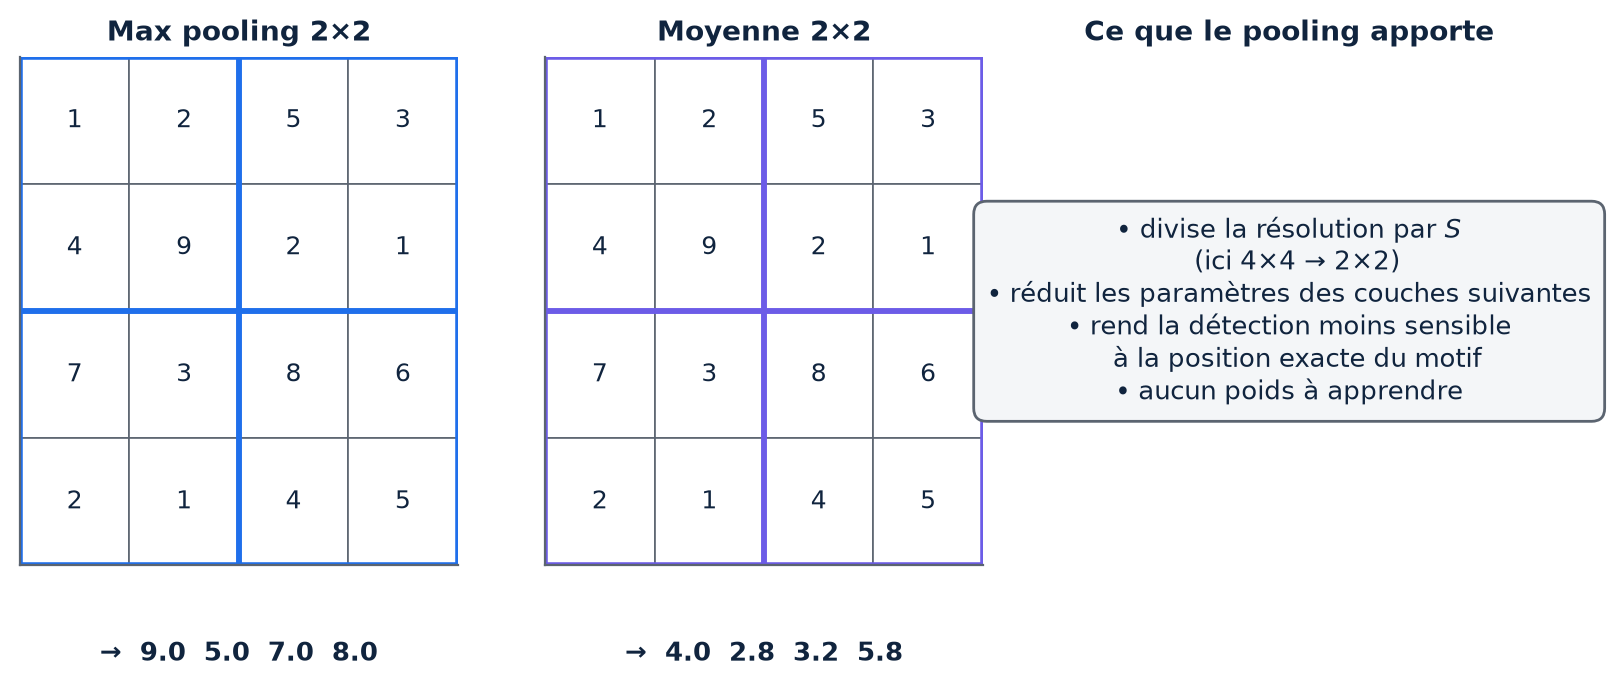
\includegraphics[width=0.82\textwidth]{h03_pooling.png}
\end{center}
\vspace{1mm}
\begin{kbox}[Ce qu'il faut retenir]
Le pooling conserve la \textbf{profondeur} (le nombre de canaux) et réduit les
deux dimensions \textbf{spatiales}. Une carte $4\times 4$ devient $2\times 2$,
mais le canal reste le même.
\end{kbox}
\end{frame}

\begin{frame}{Le pooling en pratique}
\begin{columns}[t]
\begin{column}{0.50\textwidth}
\begin{itemize}
  \item Réglages courants : fenêtre $2 \times 2$ avec pas de $2$, ou
  fenêtre $3 \times 3$ avec pas de $2$.
  \item Un pas \textbf{plus petit} que la fenêtre crée un \textbf{chevauchenment}
  et lisse davantage.
  \item Variantes : \emph{max}, \emph{moyenne}, \emph{max--moyenne}, ou
  \textbf{stride} seul (convolution à pas $2$, sans pooling).
\end{itemize}
\end{column}
\begin{column}{0.46\textwidth}
\begin{ebox}[Deux philosophies]
\begin{itemize}
  \item \textbf{Pooling explicite} (LeNet, AlexNet) : la réduction est une
  couche séparée.
  \item \textbf{Convolution à pas} (architectures modernes) : la réduction est
  intégrée à la convolution, qui apprend la manière de sous-échantillonner.
\end{itemize}
\end{ebox}
\end{column}
\end{columns}
\vspace{1mm}
\begin{wbox}[Limite du pooling]
Il \emph{détruit} de l'information : la position exacte du maximum est perdue.
C'est un défaut acceptable en classification, mais coûteux en \textbf{localisation}
(détection, segmentation) --- d'où les architectures sans pooling des chapitres suivants.
\end{wbox}
\end{frame}

\begin{frame}{Global Average Pooling : un résumé par canal}
\begin{columns}[t]
\begin{column}{0.52\textwidth}
\begin{itemize}
  \item Le \textbf{global average pooling} (GAP) fait la moyenne sur \emph{toute}
  la carte, pas sur un petit bloc.
  \item Un tenseur $5 \times 5 \times 16$ ne produit plus qu'\textbf{un nombre
  par canal} : un vecteur de $16$ valeurs.
  \item Chaque valeur résume « à quel point ce filtre a répondu » sur l'image entière.
\end{itemize}
\begin{kbox}[Le bon compte]
$5 \times 5 \times 16$ : GAP fait $25$ valeurs par canal et donne donc
$16$ nombres --- un par canal, jamais plus.
\end{kbox}
\end{column}
\begin{column}{0.44\textwidth}
\begin{ebox}[Pourquoi c'est élégant]
Placer une couche dense $16 \to 10$ après le GAP coûte
$16 \times 10 + 10 = 170$ paramètres, contre des centaines de milliers si l'on
aplatissait d'abord tout le tenseur.
\end{ebox}
\begin{wbox}[Une couche dense, si elle suivait]
Une dense sur le tenseur aplati $5\times 5\times 16 = 400$ vers $10$ classes
coûterait $400 \times 10 + 10 = 4\,010$ paramètres : $24$ fois plus.
\end{wbox}
\end{column}
\end{columns}
\end{frame}

\begin{frame}{Flatten : d'un tenseur à un vecteur}
\begin{columns}[t]
\begin{column}{0.50\textwidth}
\begin{itemize}
  \item Les couches denses n'acceptent qu'un \textbf{vecteur} : il faut déplier
  le tenseur.
  \item Opération \py{flatten} / \py{reshape} : les cartes sont mises bout à bout,
  canal par canal.
  \item La règle est simple : $H \times W \times C$ devient un vecteur de
  $H \cdot W \cdot C$ valeurs.
\end{itemize}
\begin{ebox}[Exemple chiffré]
Un tenseur $5 \times 5 \times 16$ se déplie en $5 \times 5 \times 16 = \mathbf{400}$
valeurs.
\end{ebox}
\end{column}
\begin{column}{0.46\textwidth}
\begin{wbox}[La structure spatiale disparaît]
Aplatir détruit la notion de \emph{voisinage}. C'est sans gravité ici : toute
l'information spatiale utile a déjà été extraite par les couches convolutives.
\end{wbox}
\begin{kbox}[À placer au bon endroit]
On aplatit \textbf{une seule fois}, juste avant les couches denses de décision ---
jamais au milieu du bloc convolutif.
\end{kbox}
\end{column}
\end{columns}
\end{frame}

\begin{frame}{Les couches denses : la prise de décision}
\begin{columns}[t]
\begin{column}{0.52\textwidth}
\begin{itemize}
  \item Le vecteur aplati traverse une ou deux couches denses, avec activation
  ReLU.
  \item Chaque neurone combine \emph{toutes} les valeurs : c'est une vue
  \textbf{globale} de l'image.
  \item La dernière couche dense a autant de neurones que de \textbf{classes}.
\end{itemize}
\begin{ebox}[Le coût typique du dense]
Une seule couche $1\,024 \to 1\,000$ compte
$1\,024 \times 1\,000 + 1\,000 = \mathbf{1\,025\,000}$ paramètres : plus que
toutes les couches convolutives d'un petit réseau.
\end{ebox}
\end{column}
\begin{column}{0.44\textwidth}
\begin{kbox}[Le contraste à retenir]
\begin{itemize}
  \item Convolution : peu de paramètres, vision \textbf{locale}.
  \item Dense : beaucoup de paramètres, vision \textbf{globale}.
\end{itemize}
Le CNN combine les deux : extraire localement, puis décider globalement.
\end{kbox}
\begin{wbox}[Attention au surdimensionnement]
Une couche dense trop large est la principale source de paramètres --- et donc
de surapprentissage --- dans un petit CNN.
\end{wbox}
\end{column}
\end{columns}
\end{frame}

\begin{frame}{Softmax : des scores à des probabilités}
\begin{columns}[t]
\begin{column}{0.50\textwidth}
\[
\mathrm{softmax}(z)_i = \frac{e^{z_i}}{\sum_{j} e^{z_j}}
\]
\begin{itemize}
  \item Transforme un vecteur de \textbf{scores} réels en \textbf{probabilités}
  positives qui somment à $1$.
  \item L'exponentielle accentue le score le plus grand : la classe gagnante
  ressort nettement.
  \item C'est la sortie standard d'un CNN de classification.
\end{itemize}
\end{column}
\begin{column}{0.46\textwidth}
\begin{ebox}[Exemple $\mathrm{softmax}(2,\,1,\,0)$]
$e^{2} = 7{,}389$, $e^{1} = 2{,}718$, $e^{0} = 1$ ; somme $= 11{,}107$.

\medskip
Résultat : $(0{,}6652,\ 0{,}2447,\ 0{,}0900)$.

\medskip
Le score $2$ -- le plus grand -- reçoit la probabilité la plus élevée.
\end{ebox}
\end{column}
\end{columns}
\vspace{1mm}
\begin{kbox}[Vérification]
À la sortie de la softmax, la somme des probabilités vaut exactement $1$ :
$0{,}6652 + 0{,}2447 + 0{,}0900 = 1{,}000$. C'est le test qui confirme un calcul correct.
\end{kbox}
\end{frame}

\begin{frame}{Entropie croisée : mesurer l'erreur}
\begin{columns}[t]
\begin{column}{0.52\textwidth}
\[
\mathcal{L} = -\sum_{i=1}^{C} y_i \log(\hat{p}_i)
\]
\begin{itemize}
  \item $y$ est la \textbf{vérité} (un $1$ sur la bonne classe, $0$ ailleurs).
  \item $\hat{p}$ est la prédiction de la softmax.
  \item Comme la vérité est binaire, la somme se réduit à
  $\mathcal{L} = -\log(\hat{p}_{\text{vraie}})$.
\end{itemize}
\begin{kbox}[Lecture]
L'erreur est petite quand le modèle donne une forte probabilité à la bonne
classe, et explose quand il la donne faible.
\end{kbox}
\end{column}
\begin{column}{0.44\textwidth}
\begin{ebox}[Exemples numériques]
Modèle convaincu (bonne classe) : $\hat{p} = 0{,}6652$ $\Rightarrow$
$- \ln(0{,}6652) = \mathbf{0{,}408}$.

\medskip
Toute confiance mal placée coûte lui : plus $\hat{p}$ est petit, plus l'erreur
$- \ln \hat{p}$ grandit.
\end{ebox}
\begin{wbox}[À ne pas confondre]
La softmax et l'entropie croisée sont \textbf{inseparables} en classification : la
première produit une distribution, la seconde en mesure l'écart à la vérité.
\end{wbox}
\end{column}
\end{columns}
\end{frame}

\begin{frame}[fragile]{Pooling, flatten, dense : le code}
\begin{columns}[t]
\begin{column}{0.54\textwidth}
\begin{codebox}[Les briques en PyTorch]
\begin{lstlisting}
import torch.nn as nn

pool   = nn.MaxPool2d(kernel_size=2, stride=2)
gap    = nn.AdaptiveAvgPool2d((1, 1))
flat   = nn.Flatten()
dense  = nn.Linear(in_features=400, out_features=120)

# une image fictive : 1 exemple, 16 canaux, 5x5
import torch
x = torch.zeros(1, 16, 5, 5)
x = pool(x)        # 1 x 16 x 2 x 2
x = flat(x)        # 1 x 64
\end{lstlisting}
\end{codebox}
\end{column}
\begin{column}{0.44\textwidth}
\begin{ebox}[Ce que fait chaque ligne]
\begin{itemize}
  \item \py{MaxPool2d(2,2)} : divise chaque dimension par $2$.
  \item \py{Flatten()} : déplie tout sauf la dimension de lot.
  \item \py{Linear(400,120)} : $400 \times 120 + 120$ poids et biais.
\end{itemize}
\end{ebox}
\begin{kbox}[Bon réflexe]
Toujours vérifier la forme du tenseur (\py{.shape}) après chaque brique : une
dimension fausse se paie plus tard, au moment du \py{Linear}.
\end{kbox}
\end{column}
\end{columns}
\end{frame}

\begin{frame}{Le pipeline complet d'un CNN}
\begin{center}
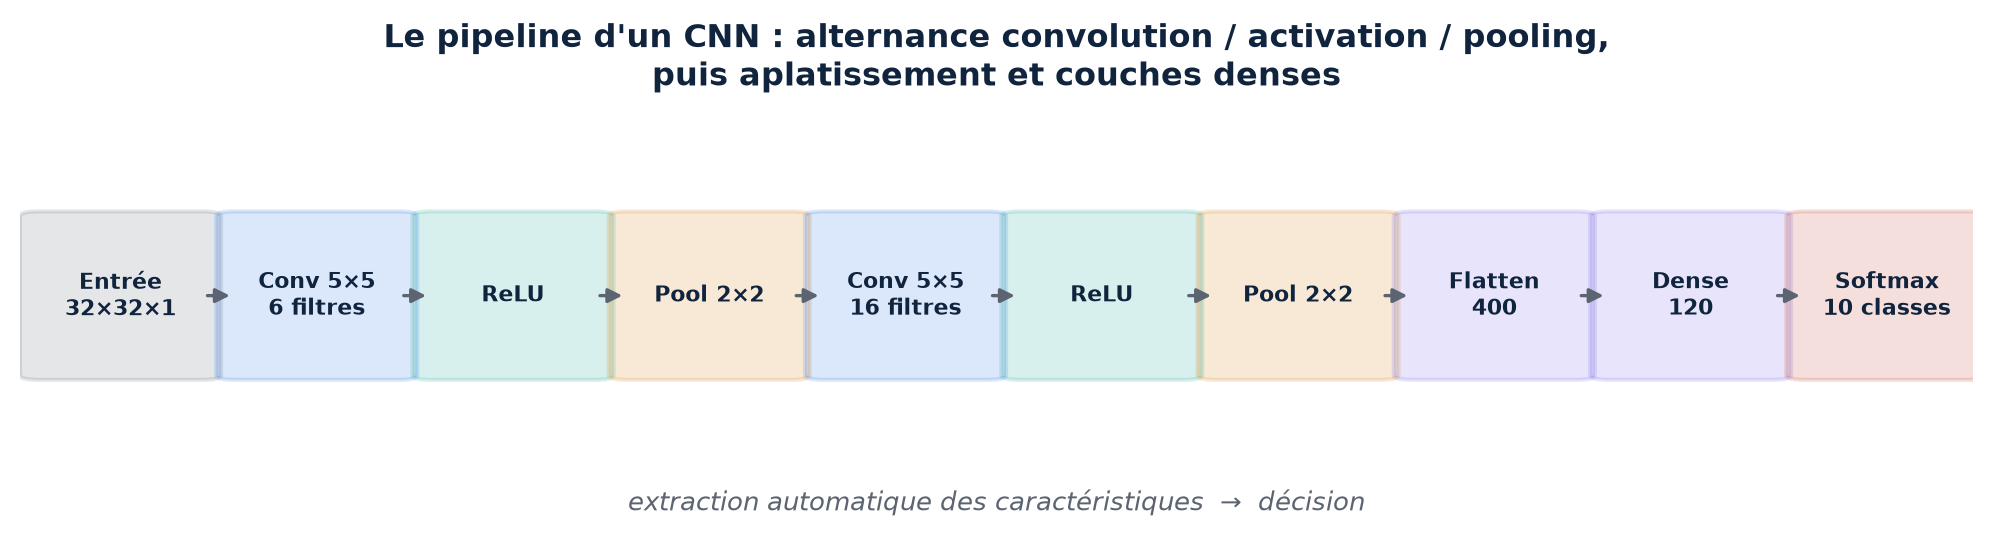
\includegraphics[width=0.92\textwidth]{h04_pipeline.png}
\end{center}
\vspace{0.5mm}
\begin{kbox}[La chaîne de traitement]
Entrée (image) $\to$ \textbf{conv} (motifs) $\to$ \textbf{ReLU} (non-linéarité)
$\to$ \textbf{pool} (résumé) $\to$ répétition $\to$ \textbf{flatten}
$\to$ \textbf{dense} (décision) $\to$ \textbf{softmax} (probabilités) $\to$ classe.
\end{kbox}
\end{frame}

\begin{frame}{Le pipeline, bloc par bloc}
\begin{columns}[t]
\begin{column}{0.50\textwidth}
\begin{center}
\begin{tabular}{@{}lll@{}}
\toprule
\textbf{Bloc} & \textbf{Rôle} & \textbf{Paramètres} \\
\midrule
conv & extraire des motifs & oui \\
ReLU & non-linéarité & non \\
pool & réduire l'espace & non \\
flatten & tenseur $\to$ vecteur & non \\
dense & classer & oui \\
softmax & produire des probas & non \\
\bottomrule
\end{tabular}
\end{center}
\end{column}
\begin{column}{0.46\textwidth}
\begin{itemize}
  \item Le motif \textbf{conv $\to$ ReLU $\to$ pool} se répète $2$ à $4$ fois.
  \item Les blocs convolutifs \textbf{extraient}, les blocs denses
  \textbf{décident}.
  \item La profondeur fait grandir le nombre de \textbf{canaux} et réduit la
  taille \textbf{spatiale}.
\end{itemize}
\begin{kbox}[Toujours vrai]
Seules \textbf{conv} et \textbf{dense} portent des paramètres appris. Toutes les
autres briques sont des règles fixes.
\end{kbox}
\end{column}
\end{columns}
\end{frame}